\documentclass[a4paper]{article}

\usepackage[utf8]{inputenc}
\usepackage[T1]{fontenc}
\usepackage[french]{babel}
\usepackage{fullpage}
\usepackage{hyperref}
\usepackage{amsmath}
\usepackage{amssymb}
\usepackage{upgreek}
\usepackage{color}
\usepackage[]{algorithm2e}
\usepackage{stmaryrd}
\usepackage{graphicx}
\usepackage{float}

\title{
    INFO-F-302 - Informatique Fondamentale\\
    \small Synthèse 2014-2015
}
\author{Florentin \bsc{Hennecker}}
\date{}

\newtheorem{theorem}{Théorème}[section]

\begin{document}
\maketitle
\tableofcontents

\section{Logique propositionnelle}

  \subsection{Coupure}
  \textit{(Les notations sont plus précises dans le cours)}\\
  $$ C_1 = p_1 \lor ... \lor p_{i-1} \lor \textcolor{red}{p} \lor 
p_{i+1} \lor ... \lor p_n$$
  $$ C_1 = s_1 \lor ... \lor s_{i-1} \lor \textcolor{red}{\lnot p} \lor 
s_{i+1} \lor ... \lor s_n$$
  \'Etant donné deux clauses $C_1$ et $C_2$ qui ont une proposition 
commune $p$
  positive dans $C_1$ et négative dans $C_2$, la règle de coupure permet 
de déduire
  la clause : 
  $$ C_3 = p_1 \lor ... \lor p_{i-1} \lor p_{i+1} \lor ... \lor p_n
     \lor s_1 \lor ... \lor s_{i-1} \lor s_{i+1} \lor ... \lor s_n$$

  On note par $C_1, C_2 \vdash^c_p C_3$ le fait que $C_3$ est déductible 
de 
  $C_1, C_2$ par coupure sur la proposition $p$.

  \paragraph{Exemple 1} $ \lnot e \lor b \lor p, \lnot p \lor a \lor b 
\vdash^c_p \lnot e \lor a \lor $
  \paragraph{Exemple 2} $ \lnot p, p, \vdash^c_p \bot $ (clause vide)

  \begin{theorem}
  Si $C_1, C_2 \vdash^c_p C_3$, alors $C_3$ est une conséquence logique 
de $C_1 \land C_2$
  \end{theorem}

  \subsubsection{Preuve par coupure}
  Une preuve par coupure est la déduction d'une clause à partir d'autres 
clauses uniquement
  en utilisant des coupures. On note par $S \vdash^c C$ le fait que $C$ 
est déductible de $S$ par coupure.

  \subsubsection{Réfutation}
  Une \textit{réfutation} d'un ensemble $S$ de clauses par coupure est 
une dérivation
  de la clause vide à partir de $S$.

  \begin{theorem}
  Si il existe une réfutation de $S$ par coupure alors l'ensemble de 
clauses $S$
  est non satisfaisable.
  \end{theorem}


% 
---------------------------------------------------------------------------- 
%
\section{Le problème SAT}

  Un problème SAT a en entrée un ensemble de clauses $S$ et en sortie la 
réponse à 
  la question : "Est-ce que $S$ est satisfaisable?". On aimerait que 
l'algorithme
  retourne une valutation $V$ qui satisfait $S$ au cas où $S$ est 
satisfaisable.
  Un solveur Sat est un programme qui décide le  problème SAT. Ces 
solveurs
  ont une complexité dans le pire cas exponentielle.

  \paragraph{Motivations}
  \begin{itemize}
    \item beaucoup de problèmes s'expriment naturellement par des 
formules en FNC.
    \item les problèmes de la classe NP se réduisent tous au problème 
SAT en temps polynomial
    \item on peut donc écrire un bon algo pour SAT plutôt qu'un bon algo 
pour chacun de ces problèmes
  \end{itemize}

  \subsection{Variantes de SAT}

    \paragraph{2-SAT} les clauses ne contiennent qu'au plus deux 
littéraux. \textbf{Solvable en temps polynomial}
    
    \paragraph{QSAT} 
    décider la satisfaisabilité de formules de la forme $\forall p_1 
\exists q_1 ... \forall p_n \exists q_n.\phi$
    où $\phi$ est une formule en CNF construite sur les propositions 
$p1, q_1, ... p_n, q_n$

    \paragraph{MAX-SAT} étant donnée une formule $\phi$ en CNF et un 
entier $k \in \mathbb{N}$, 
    peut-on satisfaire au moins $k$ clauses?

    \paragraph{WEIGHTED-MAX-SAT} on attribue des poids à chaque clause, 
on se donne
    un entier $r$ et on veut savoir si on peut satisfaire un ensemble de 
clauses dont la 
    somme des poids est au moins $r$.

  \subsection{Interprétation partielle}
  Une \textit{interprétation partielle} est un assignement noté $x/1$ ou 
$x/0$, 
  qui signifie qu'on assigne la valeur $1$ à $x$ ou la valeur $0$. Cela 
permet
  de simplifier les formules. 

    \paragraph{Exemple 1} : la formule $(x \lor y) \land (\lnot x \lor z 
\lor \lnot y)$ se simplifie
    en $z \lor \lnot y $ sous l'interprétation partielle $x/1$.\\

  On peut appliquer deux interprétations partielles à la formule $\phi$, 
ce qui se
  note ainsi : $\phi[x/b][y/b']$

    \paragraph{Exemple 2} Soit $a = x \lor y \lor z$ et $b = x \lor 
\lnot y \lor \lnot z$. Alors :
    \begin{itemize}
      \item $a[x/1] = \top$, $b[x/1] = \top$, $(a \land b)[x/1] = \top$
      \item $a[x/0] = y \lor z$
      \item $b[x/0] = \lnot y \lor \lnot z$
      \item $(a \land b)[x/0][y/0] = z$
      \item ...
    \end{itemize}

  \subsection{Proposition pivot}
  L'algorithme DPLL va essayer des interprétations partielles, la 
proposition choisie
  est la \textit{proposition pivot}. Il va successivement essayer de 
mettre la 
  proposition est vrai ou à faux, et tester récursivement la 
satisfaisabilité de formules
  simplifiées obtenues. Le choix de la proposition pivot peut évidemment 
fortement
  influencer le résultat.

  \subsubsection{Premier critère de choix}
  DPLL choisit en priorité la proposition d'une \textbf{clause unitaire} 
(un seul littéral)
  comme proposition pivot. 

  \paragraph{Exemple} Dans $x \land (y \lor \lnot z)$, $x$ est unitaire 
et doit 
  obligatoirement être interprété par $1$ pour satisfaire la formule.

  \paragraph{Exemple de propagation de clauses unitaires}
  Prenons $$\phi = (x\lor y) \land \lnot y \land (\lnot x \lor y \lor 
\lnot z)$$
  Alors $$ \phi[y/0] = x \land (\lnot x \lor \lnot z) $$
  Ce qui donne la nouvelle clause unitaire $x$ qui impose $ x = 1 $ :
  $$ \phi[y/0][x/1] =  \lnot z$$ 
  Ce qui ne contient qu'une seule clause unitaire et on obtient 
finalement :
  $$ \phi[y/0][x/1][z/0] = \top $$
  Donc $\phi$ est satisfaisable avec l'interprétation $V(x) = 1$ et 
$V(y) = V(z) = 0$

  \subsubsection{Deuxième critère de choix}
  Le deuxième critère de choix se base sur les \textbf{propositions à 
polarité unique}.

  \paragraph{Exemple} Dans la formule 
  $$\phi = (x \lor \lnot y \lor z) \land (x \lor \lnot z) \land (y \lor 
z) \land (x \lor \lnot y) $$
  $x$ apparaît toujours positivement, on peut donc directement lui 
assigner la valeur $1$
  sans être obligé de tester la valeur $0$.

  \subsection{Algorithme DPLL}
  DPLL($\phi$) retourne \texttt{VRAI} si $\phi$ est satisfaisable.

  \begin{algorithm}[H]
    \uIf{$\phi = \top$}{retourner \texttt{VRAI}}
    \uElseIf{$\phi = \top$}{retourner \texttt{FAUX}}
    \uElseIf{$\phi$ contient une clause unitaire $x$}{retourner 
DPLL($\phi[x/1]$)}
    \uElseIf{$\phi$ contient une clause unitaire $\lnot x$}{retourner 
DPLL($\phi[x/0]$)}
    \uElseIf{$\phi$ contient une proposition $x$ de polarité toujours 
positive}{retourner DPLL($\phi[x/1]$)}
    \uElseIf{$\phi$ contient une proposition $x$ de polarité toujours 
négative}{retourner DPLL($\phi[x/0]$)}
    \Else{choisir une proposition $x$ au hasard et retourner 
(DPLL($\phi[x/0]$) ou DPLL($\phi[x/1]$)) }
  \end{algorithm}

  \subsection{Transformation de Tseitin}
  Parfois, on cherche un résoudre un problème qui ne s'exprime pas 
facilement en FNC.
  La transformation de Tseitin va ajouter des nouvelles variables et des 
équivalences.

    \paragraph{Exemple} Prenons $ \phi = (p \land q) \lor \lnot (q \lor 
r) $. Dans 
    la transformation de Tseitin, on remplace $p \land q$ par $x_1$ et 
$\lnot (q \lor r)$ par $x_2$.
    Il faut donc réécrire la formule comme ceci :
    $$ (x_1 \lor x_2) \land (x_1 \leftrightarrow (p \land q)) \land (x_2 
\leftrightarrow \lnot (q \lor r) )$$
    Il reste encore à mettre les deux formules $(x_1 \leftrightarrow (p 
\land q))$ et $(x_2 \leftrightarrow \lnot (q \lor r))$ sous FNC.\\

  La technique de Tseitin sera particulièrement intéressante lorsqu'on 
devra mettre
  sous FNC des formules qui sont sous forme normale 
\textit{disjonctive}.

  \subsection{Autre exemple de rajout de variable intéressant}
  Supposons qu'on ait $n$ variables $x_0, x_1, ..., x_{n-1}$ et qu'on 
veuille
  exprimer qu'exactement une de ces variables doit être vraie. 

    \subsubsection{Solution naïve}
    On considère les deux formules suivantes en conjonction :
    \begin{itemize}
      \item \textbf{Au moins une :} $\bigvee^{n-1}_{i=0} x_i$
      \item \textbf{Au plus une :} $\bigwedge_{0 \leq i < j < n} \lnot 
x_i \lor \lnot x_j $
    \end{itemize}
    Il y a donc $\frac{n(n-1)}{2} + 1$ clauses.

    \subsubsection{Avec un encodage binaire}
    On peut faire avec $n log_2(n) + 1$ clauses (voir cours).

  \subsection{Problèmes de décision}
  On peut définir un problème de décision comme un langage de mots sur 
un alphabet
  fini $\Sigma$. On note $\Sigma^*$ l'ensemble des mots sur l'alphabet 
$\Sigma$, et
  $\epsilon$ le mot vide. Un langage sur $\Sigma$ est un sous-ensemble 
$L \subseteq \Sigma^*$. \\

  Un \textit{problème de décision} est un langage $P \subseteq 
\Sigma^*$.\\

  Chaque langage $P$ représente bien un problème dont la réponse est oui 
ou non, 
  en l'identifiant à sa fonction caractéristique $\chi_P$ :
  \begin{align*}
    \chi_P : \Sigma^* & \rightarrow & \{0,1\} \\
    u & \mapsto & \begin{cases}1 \text{si} u \in P \\ 0 \text{si} u \not 
\in P\end{cases}
  \end{align*}

  \subsection{Problème d'optimisation}
  Un \textit{problème d'optimisation} est un problème où l'on veut 
maximiser ou
  minimiser une certaine quantité. On peut associer un problème de 
décision à un
  problème d'optimisation, en donnant une borne. Si on sait résoudre le 
problème
  de décision associé à un problème d'optimisation, on peut parfois 
résoudre le
  problème d'optimisation.

  \subsection{Algorithme de décision}
  Un problème $P \subseteq \Sigma^*$ est décidé par un algorithme $A$ si 
pour 
  tout mot $u \in \Sigma^*$ : 
  \begin{itemize}
    \item $A$ termine et retourne 1 si $u \in P$
    \item $A$ termine et retourne 0 si $u \not \in P$
  \end{itemize}

  \subsection{La classe $\mathcal{P}$}
  La classe $\mathcal{P}$ est la classe des problèmes pouvant être 
décidés en temps
  polynomial. Plus précisément, un problème $P \subseteq \Sigma^*$ est 
dans $\mathcal{P}$
  si il existe un algorithme $A$ et une constante $k$ tel que pour tout 
mot $u$
  de longueur $n$, 
  \begin{itemize}
    \item $A$ retourne 1 en temps $O(n^k)$ si $u \in P$
    \item $A$ retourne 0 en temps $O(n^k)$ si $u \not \in P$
  \end{itemize}

  Exemples :
  \begin{itemize}
    \item décider si un tableau est trié
    \item décider si un entier codé en binaire est premier (difficile, 
problème
    resté ouvert pendant longtemps)
  \end{itemize}

  \subsection{Algorithme de vérification}
  Informellement, un algorithme de vérification est un algorithme qui, 
étant donnée
  une solution candidate à un problème de décision, décide si oui ou non 
cette
  solution est valide. Formellement : \\

  Un algorithme de vérification pour un problème $P \subseteq \Sigma^*$ 
est un
  algorithme $A$ prenant deux mots en argument, tel que 
  $$ P = \{ u \in \Sigma^* | \exists v \in \Sigma^*, A(u,v) =1 \} $$
  Lorsque $A(u,v) = 1$, $v$ est appelé un certificat pour $u$.

  \subsection{La classe $\mathcal{N}\mathcal{P}$}
  La classe $\mathcal{N}\mathcal{P}$ est la classe des problèmes pouvant 
être vérifiés
  en temps polynomial. Note : $\mathcal{P} \subseteq 
\mathcal{N}\mathcal{P} \subseteq$ ExpTime.\\

  La \textbf{grande conjecture} de l'informatique fondamentale est :
  $$ \mathcal{P} \neq \mathcal{N}\mathcal{P} $$

  Un problème de décision $P$ est $\mathcal{N}\mathcal{P}$-complet si il 
est dans
  $\mathcal{N}\mathcal{P}$ et tout autre problème $P'$ de 
$\mathcal{N}\mathcal{P}$
  se réduit à $P$ en temps polynomial.


% 
---------------------------------------------------------------------------- 
%
\section{La logique des prédicats}
  En logique des prédicats,
  \begin{itemize}
    \item on ajoute les quantificateurs
    \item on généralise les valeurs que peuvent prendre les variables
    \item on ajoute des relations (appelées prédicats) pour décrire 
certaines
    relations entre ces valeurs
    \item on ajoute des symboles de fonction à la syntaxe
  \end{itemize}

  \paragraph{Exemple} $\forall x\forall y . PremierEntreEux(x,y) 
\leftrightarrow \exists x' \exists y' . x.x'+y.y' = 1$\\

  Les ingrédients pour construire les formules sont : connecteurs 
Booléens,
  quantificateurs, symboles de relations, de fonctions, constantes et 
termes. Pour
  satisfaire une formule, il faudra définir une interprétation des 
symboles dans un domaine.

  \subsection{Langages du premier ordre}
  Un \textit{langage $\mathcal{L}$} de la logique du premier ordre est 
caractérisé par
  \begin{itemize}
    \item{des symboles de relations ou prédicats, notés $p, q, r, s, 
...$}
    \item{des symboles de fonctions, notés $f, g, h, ...$}
    \item{des symboles de constantes, notés $c, d, e, ...$}
  \end{itemize}
  \'A chaque prédicat $p$ (resp. fonction $f$), on associe un entier 
strictement
  positif appelé l'\textit{arité} de $p$ (resp $f$), c'est-à-dire le 
nombre
  d'arguments de $p$ (resp $f$). On notera parfois $p|_n$ $f|_n$.\\

  On utilise le prédicat "=" pour dénoter l'égalité. Si "=" fait partie 
du 
  vocabulaire du langage $\mathcal{L}$, on dit que $\mathcal{L}$ est 
égalitaire.

  \paragraph{Exemples} 
  $$\mathcal{L}_1 = \{ r|_1, c \}$$
  $$\mathcal{L}_2 = \{ r|_2, f|_1, g|_2, h|_2, c, d \}$$

  L'ensemble des \textit{termes d'un langage $\mathcal{L}$}, noté 
$\mathcal{T}$ est le plus petit
  ensemble qui contient les symboles de constantes et de variables et 
qui est
  clos par application des fonctions.

  \paragraph{Exemples}
  \begin{itemize}
    \item les seuls termes du langage $\mathcal{L}_1$ sont la constante 
$c$ et les variables
    \item les expressions suivantes sont des termes du langage 
$\mathcal{L}_2$ : $f(c)$, $f(h(f(c),d))$, $f(y)$,...
  \end{itemize}
  Un terme est \textit{clos} s'il est sans variable. $f(c)$ est clos.\\

  L'ensemble des \textit{formules atomiques} d'un langage $\mathcal{L}$ 
est l'ensemble
  des formules de la forme :
  \begin{itemize}
    \item $p(t_1, t_2, ..., t_n)$ où $p$ est un prédicat d'arité $n$ et 
$t_1, t_2, ..., t_n$ 
    sont des termes du langage $\mathcal{L}$
    \item $t_1 = t_2$ si $\mathcal{L}$ est égalitaire et $t_1, t_2$ sont 
des termes
    du langage $\mathcal{L}$
  \end{itemize}

  L'ensemble des \textit{formules du langage $\mathcal{L}$}, que l'on 
désigne par
  $\mathcal{F}(\mathcal{L})$ est défini par la grammaire suivante :
  $$ \phi ::= p(t_1, t_2,...,t_n) | \phi \land \phi | \phi \lor \phi | 
\lnot \phi | \phi \rightarrow \phi | \phi \leftrightarrow \phi | \exists 
x.\phi | \forall x.\phi | (\phi) $$

  Toute formule d'un langage du premier ordre se décompose de manière 
unique sous
  l'une, et une seule, des formes suivantes :
  \begin{itemize}
    \item une formule atomique
    \item $\lnot \phi$, où $\phi$ est une formule,
    \item $\phi \land \psi$, $\phi \lor \psi$, $\phi \rightarrow \psi$, 
$\phi \leftrightarrow \psi$
    où $\phi$ et $\psi$ sont des formules
    \item $\forall x. \phi$ ou $ \exists x.\phi$ où $\phi$ est une 
formule et $x$ une variable.
   \end{itemize}

   \paragraph{Occurences}
   Une \textit{occurence} d'une variable dans une formule est un couple 
constitué
   de cette variable et d'une place effective, c'est-à-dire qui ne suit 
pas 
   un quantificateur. \textbf{Exemple :} dans $r(x,z) \rightarrow 
\forall z.(r(y,z) \lor y = z)$,
   la variable $x$ possède une occurence, la variable $y$ deux et $z$ 
trois.

   Une occurence d'une variable $x$ dans une formule $\phi$ est une 
\textit{occurence libre}
   si elle ne se trouve dans aucune sous-formule de $\phi$, qui commence 
par une
   quantification $\forall x$ ou $\exists x$. Dans le cas contraire, 
l'occurence
   est dite \textit{liée}. Une variable est libre dans une formule si 
elle a 
   au moins une occurence libre dans cette formule. Une formule close 
est une formule
   sans variable libre.

   \subsubsection{Structures}
   Une \textit{structure $\mathcal{M}$} pour un langage $\mathcal{L}$ se 
compose
   d'un ensemble non vide $M$, appelé le \textit{domaine} et d'une 
interprétation des
   symboles de prédicats par des relations sur $M$, des symboles de 
fonctions
   par des fonctions de M, et des constantes par des éléments de M. Plus 
précisément:

   \begin{itemize}
     \item d'un sous ensemle de $M^n$, noté $r^{\mathcal{M}}$, pour 
chaque symbole
     de prédicat $r$ d'arité $n$ dans $\mathcal{L}$
     \item d'une fonction de $M^n$ dans $M$, notée $f^{\mathcal{M}}$, 
pour chaque symbole
     de fonction $f$ d'arité $m$ dans $\mathcal{L}$
     \item d'un élément de $M$, noté $r^{\mathcal{M}}$, pour chaque 
symbole de 
     constante $c$ dans $\mathcal{L}$
   \end{itemize}

   \paragraph{Exemple} L'ensemble des réels $\mathbb{R}$ permet de 
construire une 
   structure pour $\mathcal{L}_2 = \{r, f, g, h, c, d\}$ de la façon 
suivante:

   \begin{itemize}
     \item on interprète le prédicat $r$ comme l'ordre $\leq$ sur les 
réels
     \item on interprète $f$ comme la fonction $+1$, $g$ comme $+$ et 
$h$ comme $\times$
     \item on interprète les constantes $c$ et $d$ comme $0$ et $1$
   \end{itemize}
   Cette structure se note $$ \mathcal{M}_2 = (\mathbb{R}, \leq, +1, +, 
\times, 0, 1) $$ 


% 
---------------------------------------------------------------------------- 
%
\section{Preuves de programmes}
  \subsection{Triplets de Hoare}
  Informellement, les triplets de Hoare sont de la forme $(\phi, P, 
\psi)$ où $P$
  est un programme, $\phi$ (resp $\psi$) est une pré-condition (resp. 
post-condition) 
  décrite par une formule de la logique du premier ordre. On notera en 
général $\llparenthesis \phi\rrparenthesis P \llparenthesis 
\psi\rrparenthesis $.
  Nous allons définir un système de preuve pour démontrer que, supposant 
que $\phi$
  est satisfaite, $\psi$ est satisfaite aussi après exécution du 
programme $P$.

  \subsection{Correction}
  Soit $\phi$ une condition (pré ou post) et $I:x\rightarrow \mathbb{Z}$ 
un état. 
  On dit que $I$ \textit{satisfait} $\phi$, noté $I \vDash \phi$, si 
$\mathbb{Z}, I \vDash \phi$.\\

  On dit qu'un triplet $\llparenthesis \phi\rrparenthesis 
P\llparenthesis \psi\rrparenthesis $ est \textit{partiellement 
satisfait} si
  pour tout état qui satisfait $\phi$, l'état résultant de l'exécution 
de $P$
  satisfait $\psi$, pourvu que $P$ termine. On note cette relation 
$\vDash_{par} \llparenthesis \phi\rrparenthesis P\llparenthesis 
\psi\rrparenthesis $.\\

  On dit qu'un triplet $\llparenthesis \phi\rrparenthesis 
P\llparenthesis \psi\rrparenthesis $ est \textit{satisfait} si
  pour tout état qui satisfait $\phi$, l'exécution de $P$ à partir de 
cet état termine
  et l'état résultant de cette exécution satisfait $\psi$. On note cette 
relation $\vDash \llparenthesis \phi\rrparenthesis P\llparenthesis 
\psi\rrparenthesis $.

  \subsection{Système de preuve $\vdash_{par}$}

  \paragraph{Composition}
  $$ \frac{\llparenthesis \phi\rrparenthesis C_1\llparenthesis 
\eta\rrparenthesis \quad \llparenthesis \eta\rrparenthesis 
C_2\llparenthesis \psi\rrparenthesis }{\llparenthesis \phi\rrparenthesis 
C_1;C_2 \llparenthesis \psi\rrparenthesis }Composition $$

  \paragraph{Assignation}
  $$ \frac{}{\llparenthesis \psi[E/x] \rrparenthesis x:=E \llparenthesis 
\psi \rrparenthesis}Assignation $$
  où $\psi[E/x]$ est la formule $\psi$ où on a remplacé toutes les 
occurences de $x$ par $E$.
  Cette règle est un axiome. \textbf{Exemple :} $\llparenthesis y+z \geq 
0 \rrparenthesis x:= y+z \llparenthesis x \geq 0 \rrparenthesis$

  \paragraph{Si-Alors}
  $$  \frac{
        \llparenthesis \phi \land B \rrparenthesis C_1 \llparenthesis 
\psi \rrparenthesis \quad
        \llparenthesis \phi \land \lnot B \rrparenthesis C_2 
\llparenthesis \psi \rrparenthesis
      }
      {
        \llparenthesis \phi \rrparenthesis\, \texttt{if}\, B\, \{ C_1 
\}\, \texttt{else}\, \{ C_2\}\, \llparenthesis \psi \rrparenthesis
      } Si-Alors
  $$ 

  \paragraph{Implication}
  $$
    \frac{
      \phi' \vDash \phi \quad \llparenthesis\phi\rrparenthesis C 
\llparenthesis\psi\rrparenthesis \quad \psi \vDash \psi'
    }
    {
      \llparenthesis\phi'\rrparenthesis C 
\llparenthesis\psi'\rrparenthesis
    } Implication
  $$
  On pourra omettre une des implications si on n'a besoin que de l'une 
ou des deux.

  \paragraph{While Partiel}
  $$
    \frac{
      \llparenthesis\psi \land B \rrparenthesis C 
\llparenthesis\psi\rrparenthesis
    }
    {
      \llparenthesis\psi\rrparenthesis\, \texttt{while}\, B\, \{C\}\, 
\llparenthesis\psi \land \lnot B \rrparenthesis
    } WhilePar
  $$
  La propriété $\psi$ est appelée \textit{invariant}. Elle est toujours 
vraie à chaque
  passage dans la boucle, ainsi qu'après le dernier passage.

  \subsection{Correction et complétude}
  Soit $\llparenthesis\phi\rrparenthesis P 
\llparenthesis\psi\rrparenthesis$ un triplet
  de Hoare. Alors $\vDash_{par} \llparenthesis\phi\rrparenthesis P 
\llparenthesis\psi\rrparenthesis$
  si et seulement si $\vdash_{par} \llparenthesis\phi\rrparenthesis P 
\llparenthesis\psi\rrparenthesis$

  \subsection{Terminaison d'un programme}
  Comme l'instruction \texttt{while} est la seule source de 
non-terminaison,
  on va identifier une expression arithmétique $E$ et démontrer qu'elle
  décroît strictemenet à chaque passage dans la boucle. Comme la 
quantité ne peut
  être négative, on aura bien une preuve de terminaison. \\

  Une telle expression est appelée \textit{variant}.

  \paragraph{While Total}
  $$
    \frac{
      \llparenthesis\eta\land B \land 0 \leq E = e_0 \rrparenthesis
      C
      \llparenthesis\eta\land 0 \leq E < e_0 \rrparenthesis
    }
    {
      \llparenthesis\eta\land 0 \leq E = e_0 \rrparenthesis\,
      \texttt{while}\, B\, \{C\}\,
      \llparenthesis\eta\land\lnot B\rrparenthesis
    } WhileTot
  $$
  \begin{itemize}
    \item $E$ est l'expression arithmétique qui décroît à chaque 
exécution de $C$
    \item $e_0$ est une variable logique
    \item $\eta$ est l'invariant
  \end{itemize}


% 
---------------------------------------------------------------------------- 
%
\section{Automates finis}
  Un automate fini lit une séquence de lettres de gauche à droite, 
possède un 
  nombre fini d'états. En fonction de l'état courant et de la lettre 
lue, il se
  déplace vers un autre état.\\

  L'état initial est représenté par une flèche sans source et les états 
finaux
  sont représentés par des doubles cercles. Le mot est accepté si et 
seulement si
  l'automate se trouve dans un état final à la fin du mot.

  \begin{figure}[H]
    \begin{center}
      \includegraphics[width=0.3\textwidth]{fsa/fsa1.eps}
      \caption{Automate fini $A$}
      \label{fig:fsa:1}
    \end{center}
  \end{figure}

  \paragraph{Langage accepté} Le \textit{langage accepté (ou reconnu)} 
par
  l'automate $A$ (fig. \ref{fig:fsa:1}), noté $L(A)$, est l'ensemble des 
mots
  qui contiennent un nombre pair de lettres $a$ :
  $$ L(A) = \{ w \in \{a,b\}^* | w\, \text{contient un nombre pair de} a 
\}$$

  \paragraph{Définition formelle} Un automate fini $A$ sur un alphabet 
$\Sigma$
  est un 4-uplet $(Q, q_0, F, \delta)$ où
  \begin{itemize}
    \item $Q$ est un ensemble fini d'éléments appelés \textit{états}
    \item $q_0$ est appelé \textit{état initial}
    \item $F \subseteq Q$ est un ensemble d'états dits \textit{finaux ou 
acceptants}
    \item $\delta : Q \times \Sigma \rightarrow Q $ est une fonction 
(pas nécessairement totale)
    appelée \textit{fonction de transition}
  \end{itemize}

  \paragraph{Exécution} Une \textit{exécution} de $A$ est une suite 
finie 
  $e = p_0 \sigma_1 p_1 \sigma_2 ... p_{n-1} \sigma_n p_n$ ($n \geq 0$) 
telle que
  \begin{itemize}
    \item $p_0 = q_0$
    \item $\forall i \in \{0,...,n\} : p_i \in Q$
    \item $\forall i \in \{1,...,n\} : \sigma_i \in \Sigma$
    \item $\forall i \in \{0,...,n-1\} : \delta(p_i, \sigma_{i+1})$ est 
définie
    et vaut $p_i+1$
  \end{itemize}
  On dit que l'exécution $e$ est \textit{acceptante} si l'état atteint 
est final ($p_n \in F$)

  \paragraph{Complétion} Un automate $A$ est dit \textit{complet} si sa 
fonction de
  transition est totale.\\

  \textbf{Lemme} On peut toujours transformer un automate $A$ en un 
automate $B$
  complet qui accepte le même langage. (Idée : ajouter un état 
supplémentaire 
  appelé état puits non final et ajouter les transition manquantes vers 
cet état)

  \subsection{Test du vide}
  Le problème VIDE est le suivant :
  \begin{itemize}
    \item \textbf{Entrée :} un automate $A$ sur un alphabet $\Sigma$
    \item \textbf{Sortie :} est-ce que $L(A) = \varnothing$ ?
  \end{itemize}

  \paragraph{Etats atteignables} Soit $A = (Q, q_0, F, \delta)$ un 
automate sur un
  alphabet $\Sigma$. Un état $q\in Q$ est dit \textit{atteignable} s'il 
existe
  un mot $w \in \Sigma^*$ et une exécution de $A$ sur $w$ qui se termine 
en $q$.\\

  Etant donné un automate $A$ avec $n$ états et $m$ transitions, on peut 
tester
  en $O(n+m)$ si $L(A) \neq \varnothing$ (en utilisant des algorithmes 
de graphe
  classiques comme le parcours en largeur par exemple).

  \subsection{Opérations Booléennes sur les langages}
  \paragraph{Complément de $L \subseteq \Sigma^*$ :} $\overline{L} = \{ 
w \in \Sigma^* | w \not \in L\} = \Sigma^* \setminus L$.

  \paragraph{Union, Intersection :} Trivial.

  \subsection{Clôture des automates par opérations Booléennes}
  Soient $A_1$ et $A_2$ des automates finis sur un alphabet $\Sigma$. Il 
existe
  des automates $A_c$, $U$ et $I$ tels que :
  \begin{center}
    \begin{align*}
      L(A_c) & = \overline{L(A_1)}\\
      L(U) & = L(A_1) \cup L(A_2)\\
      L(I) & = L(A_1) \cap L(A_2)
    \end{align*}
  \end{center}

  \subsubsection{Clôture par complément}
  Si $A = (Q, Q_0, F, \delta)$ n'est pas complet, il faut le compléter, 
puis
  $A_c = (Q, Q_0, Q \setminus F, \delta)$. Par exemple, si $A = $

  \begin{figure}[H]
    \begin{center}
      \includegraphics[width=0.3\textwidth]{fsa/fsa1.eps}
    \end{center}
  \end{figure}

  alors $A_c =$

  \begin{figure}[H]
    \begin{center}
      \includegraphics[width=0.3\textwidth]{fsa/fsa1_complement.eps}
    \end{center}
  \end{figure}

  \subsubsection{Produit d'automates}
  On appellera \textit{pré-automate} sur $\Sigma$ un triplet $(Q, q_0, 
\delta)$
  où $Q$ est un ensemble fini, $q_0 \in Q$ et $\delta : Q \times \Sigma 
\rightarrow Q$
  est une fonction.\\

  Soient $A_1 = (Q_1, q_0^1, F_1, \delta_1$ et $A_2 = (Q_2, q_0^2, F_2, 
\delta_2$
  deux automates sur $\Sigma$. Le produit de $A_1$ et $A_2$, noté $A_1 
\otimes A_2$
  est le pré-automate défini par : 
  $$ A_1 \otimes A_2 = (Q_1 \times Q_2, (q_0^1, q_0^2), \delta_{12})$$
  où, pour tout $(q_1, q_2) \in Q_1 \times Q_2$, pour tout $\sigma \in 
\Sigma$,

  \begin{center} 
    \begin{align*} 
     \delta((q_1, q_2), \sigma) = 
      \begin{cases}
        \text{indéfini} & \text{si}\, \delta_1(q_1, \sigma)\, \text{est 
indéfinie}\\
        \text{indéfini} & \text{si}\, \delta_2(q_2, \sigma)\, \text{est 
indéfinie}\\
        (\delta_1(q_1, \sigma), \delta_2(q_2, \sigma)) & \text{sinon}.
      \end{cases} 
    \end{align*} 
  \end{center} 

  \paragraph{Exemple} Voici un exemple graphique

  \begin{figure}[H]
    \begin{center}
      \begin{minipage}{0.45\textwidth}
        \includegraphics{fsa/fsa_productA1.eps}
        \caption{$A_1$}
      \end{minipage}\hfill
      \begin{minipage}{0.45\textwidth}
        \includegraphics{fsa/fsa_productA2.eps}
        \caption{$A_2$}
      \end{minipage}
    \end{center}
  \end{figure}

  \begin{figure}[H]
    \begin{center}
      \includegraphics[width=0.5\textwidth]{fsa/fsa_product.eps}
      \caption{$A_1 \otimes A_2$}
    \end{center}
  \end{figure}

  \paragraph{Exemple intuitif} Si $L(A_1)$ est l'ensemble des mots qui 
contiennent
  un nombre pair de $b$ et $L(A_2)$ l'ensemble des mots qui contiennent 
un 
  nombre pair de $a$, toute exécution de $A_1 \otimes A_2$ sur un mot 
$w$ simule
  en parallèle l'exécution de $A_1$ sur $w$, ainsi que celle de $A_2$.

  \subsubsection{Intersection et Union}
  \begin{itemize}
    \item Pour avoir $L(A_1) \cap L(A_2)$, il suffit de prendre $F_\cap 
= F_1 \times F_2$
    pour états finaux de $A_1 \otimes A_2$
    \item Pour avoir $L(A_1) \cup L(A_2)$, il suffit de prendre $F_\cup 
= (F_1 \times Q_2) \cup (Q_1 \times F_2)$
    pour états finaux de $A_1 \otimes A_2$
  \end{itemize}
  Pour la clôture (construire un automate à partir du pré-automate 
produit et des états
  finaux ci-dessus), $A_1$ et $A_2$ doivent être complets.

  \subsubsection{Inclusion et Equivalence}
  Soient $A_1$ et $A_2$ deux automates sur un alphabet $\Sigma$. On dit 
que
  $A_1$ et $A_2$ sont équivalents si $L(A_1) = L(A_2)$.\\
  On peut décider en temps polynomial si $L(A_1) \subseteq L(A_2)$, et 
si $L(A_1) = L(A_2)$

  \paragraph{Algorithme}
  $L(A_1) = L(A_2)$ ssi $L(A_1) \subseteq L(A_2)$ et $L(A_2) \subseteq 
L(A_1)$.
  On peut donc se concentrer sur l'inclusion. Il faut compléter $A_1$ et 
$A_2$.
  Ensuite, on a $L(A_1) \subseteq L(A_2)$ ssi $L(A_1) \cap 
\overline{L(A_2)} = \varnothing$
  \begin{enumerate}
    \item construire $A_c$ tel que $L(A_c) = \overline{L(A_2)}$
    \item construire $I$ tel que $L(I) = L(A_1) \cap L(A_c)$ avec le 
produit $A_1 \otimes A_c$
    \item tester le vide de $I$
  \end{enumerate}

  \paragraph{Exemple} Il y a un excellent exemple dans le cours.


  \subsection{Minimisation}
  Etant donné un automate $A$, l'objectif de la minimisation est de 
construire un automate
  complet $M$ tel que $M$ a un nombre d'états minimal, et $M$ est 
équivalent à $A$.

  \subsubsection{Relation de Myhill-Nerode}
  Soit $L \subseteq \Sigma^*$ un langage, et $u,v\in L$ deux mots de 
$L$.
  Les mots $u$ et $v$ sont dits équivalents pour $L$, noté $u \equiv_L 
v$ si
  $ \forall w \in \Sigma^*, uw \in L \text{ssi} vw \in L$.

  \paragraph{Exemple} les mots $u=ababb$ et $v=baa$ sont équivalents 
pour le 
  langage PAIR.

  \paragraph{Proposition} La relation $\equiv_L$ est une relation 
d'équivalence. 
  (symétrique, réflexive, transitive)

  \paragraph{Classes d'équivalence}
  Etant donné un mot $u \in \Sigma^*$, la \textit{classe d'équivalence} 
de $u$ pour
  $\equiv_L$, notée $[u]_L$, est l'ensemble des mots équivalents à $u$ :
  $$ \forall u \in \Sigma^*, [u]_L = \{v \in \Sigma^* | u \equiv_L v\}$$
  On note $\Sigma^*/_{\equiv_L}$ l'ensemble quotient de $\Sigma^*$ par 
$\equiv_L$, 
  i.e. l'ensemble des classes d'équivalences.

  \subsubsection{Théorème de Myhill-Nerode}
  Soit $L \subseteq \Sigma^*$. Alors $L$ est reconnaissable par un 
automate 
  ssi $\Sigma^*/_{\equiv_L}$ est un ensemble fini.
  
  \paragraph{Exemple} Avec le langage PAIR, on a exactement deux classes 
d'équivalences:
  \begin{align*}
    \{a,b\}^*/_{\equiv_{PAIR}} & = \{ \{\epsilon, aa, aba, baa,...\},\, 
\{a, ab, ba, aaa,...\} \}\\
    & = \{[\epsilon]_{\equiv_{PAIR}}, [a]_{\equiv_{PAIR}}\}
  \end{align*}

  \subsubsection{Automate Quotient}
  Soit $L \subseteq \Sigma^*$ un langage reconnaissable par un automate. 
  Donc $\Sigma^*/_{\equiv_L}$ est un ensemble fini.\\

  L'\textit{automate quotient} de $L$ est l'automate complet $A_L = (Q, 
q_0, F, \delta)$ où
  \begin{itemize}
    \item $Q = \Sigma^*/_{\equiv_L}$
    \item $q_0 = [\epsilon]_L$
    \item $F = \{ [u]_L\, |\, u \in L \}$
    \item $\delta$ est la fonction de transition définie par 
$\delta([u]_L, a) = [ua]_L$
  \end{itemize}

  \paragraph{Théorème} Soit $L \subseteq \Sigma^*$. L'automate quotient 
$A_L$ est
  le plus petit automate complet (en nombre d'états) qui reconnaît $L$, 
et il est 
  unique (modulo renommage des états).

  \subsubsection{Calcul de l'automate minimal}
  \paragraph{Définitions}
  Soit $A = (Q, q_0, F, \delta)$ un automate complet sur un alphabet 
$\Sigma$. 
  Pour tout mot $u \in \Sigma^*$, pour tout état $q \in Q$, n note :
  \begin{itemize}
    \item $q \cdot u$ l'état atteint par $A$ après lecture de $u$ à 
partir de $q$
    (il existe car $A$ est complet)
    \item $L_q$ le langage formé des mots $u$ tels que $q\cdot u \in F$ 
(les mots
    acceptés à partir de $q$).
    \item $\forall p,q\in Q$, $p \equiv_A q$ si $L_p = L_q$
  \end{itemize}

  \paragraph{Proposition} Soit $A$ un automate complet. Alors pour tout 
$u,v \in \Sigma^*$,
  $u \equiv_{L(A)} v$ ssi $q_0 \cdot u \equiv_A q_O \cdot v$.

  \paragraph{Calcul}
  \begin{itemize}
    \item Il suffit de calculer les classes d'équivalences de $Q$ pour 
$\equiv_A$, 
    ce qui donnera les états
    \item la classe de $q_0$ est l'état initial
    \item toute classe qui contient un état final est finale (en fait, 
si une classe
    contient un état final, alors tous ces états sont finaux)
    \item on met une transition de l'état $[q]_{\equiv_A}$ à l'état $[q 
\cdot a]_{\equiv_A}$,
    en lisant $a$, pour tout $a \in \Sigma$, et tout $q \in Q$.
  \end{itemize}
  
  \paragraph{Proposition} Si $p \equiv_A q$, alors $p \cdot q \equiv_A q 
\cdot a$ pour tout $a \in \Sigma$.


  \subsection{Expressions Rationnelles}
  Une \textit{expression rationnelle} $E$ sur un alphabet $\Sigma$ est 
une expression
  qui respecte la grammaire suivante :
  $$ E\; ::=\; \epsilon\,|\, a\,|\,\varnothing\,|\, (E+E)\,|\, (E.E) 
\,|\, E^* $$

  \subsubsection{Autres opérations sur les langages}
  Soient $L, L_1, L_2, \subseteq \Sigma^*$ trois langages. Alors
  \begin{itemize}
    \item $L_1.L_2 = \{u_1u_2\, |\, u_1 \in L_1 \land u_2 \in L_2\}$ (on 
écrira aussi $L_1L_2$)
    \item $L^* = \{u^n\, |\, u \in L \land n \geq 0\}$ (en particulier 
$\epsilon \in L^*$ si $L \neq \varnothing$)
  \end{itemize}

  \subsubsection{Sémantique}
  La sémantique d'une expression rationnelle $E$ sur $\Sigma$ est donnée 
par un 
  langage, noté $L(E)$, défini inductivement par :
  \begin{itemize}
    \item $L(\epsilon) = \{\epsilon\}$
    \item $L(a) = \{a\}$ pour tout $a \in \Sigma$
    \item $L(\varnothing) = \varnothing$
    \item $L((E_1+E_2)) = L(E_1) \cup L(E_2)$
    \item $L((E_1.E_2)) = L(E_1) . L(E_2)$
    \item $L(E^*) = L(E)^*$
  \end{itemize}

  \paragraph{Exemples} Sur $\Sigma = \{a,b\}$.
  \begin{itemize}
    \item $L((a+b)^*a(a+b)^*)$ est l'ensemble des mots qui contiennent 
au moins un $a$
    \item $L(a^*b^*)$ est l'ensemble de mots qui sont des séquences de 
$a$ suivies 
    de séquences de $b$.
  \end{itemize}

  \subsubsection{Théorème dit de Kleene}
  La classe des langages définissables par automates, et la classe des 
langages
  définissables par expressions rationnelles, sont les mêmes. Autrement 
dit, si 
  $L \subseteq \Sigma^*$ est un langage, alors il existe un automate $A$ 
tel
  que $L = L(A)$ ssi il existe une expression rationnelle $E$ telle que 
$L = L(E)$.\\

  \paragraph{Remarque} Il existe un algorithme qui transforme tout 
automate
  en expression rationnelle et inversement.

\end{document}
